\chapter{Theoretische Einführung}



\section{Grundlagen des 3D-Drucks mittels selektivem Laserschmelzen (SLM)}
	Die \emph{additive Fertigung} (AM) spielt in unserem Leben eine immer größere Rolle. Während
	sich bereits ein Hobbymarkt für preisgünstige 3D-Drucker im eigenen Haushalt etabliert hat,
	ist die industrielle Anwendung nicht zu vernachlässigen. Eine von Essentium, einem Hersteller
	von industriellen 3D-Druckern und Materialien, angefertigte Umfrage zeigte, dass sich die
	Anzahl der Firmen, die 3D-Druck zur industriellen Fertigung benutzen, von 2018 auf 2019 fast
	verdoppelte. Während der Anteil 2018 noch bei 21\% lag, änderte er sich innerhalb eines Jahres
	auf 40\% \cite{stevenson2019survey}.

	Obwohl es eine Vielzahl unterschiedlicher Methoden der additiven Fertigung gibt, funktionieren
	alle nach einem ähnlichen Grundprinzip: Das digitale 3-dimension\-ale Modell wird durch einen
	sogenannten \emph{Slicer} in Schnittebenen unterteilt, die vom 3D-Drucker nacheinander
	produziert und aufgeschichtet werden.

	%\subsection{Funktionsweise und Unterschiede zu anderen Methoden}
	\subsection{Funktionsweise und Unterschiede zum bekannteren FDM-Druck}
		Das vermutlich bekannteste Verfahren zur additiven Fertigung ist wahrscheinlich das
		\emph{Fused Depositing Modeling} (FDM), aus Markenrechtsgründen auch bekannt als
		\emph{Fused Filament Fabrication} (FFF). Dabei wird ein Kunststofffilament geschmolzen
		und durch eine Düse extrudiert. Die Düse (\emph{Hotend}) fährt hierbei während des
		Extrudierens wie in Abbildung \ref{fig:fdm} dargestellt die Schnittebene ab, sodass
		Ebene für Ebene das gewünschte Objekt aufgeschichtet wird. Schichtdicken sind bei diesem
		Verfahren üblicherweise zwischen \SI{0,025}{\milli\meter} und \SI{1,25}{\milli\meter}
		\cite{wikipedia2021fused}.

		Obwohl dieses Verfahren relativ einfach umzusetzen ist, wird es durch verschiedene
		Faktoren limitiert. So ist beispielsweise für die Qualität die Form des zu druckenden
		Objekts relevant. Außerdem ist dieses Verfahren auf bestimmte Materialien beschränkt, wie
		Thermoplaste und Formwachse. Die Druckbarkeit wird nicht zuletzt auch durch die
		Gravitation beschränkt, sodass je nach Form auch Stützstrukturen (\emph{support}, siehe
		Abbildung \ref{fig:fdm}) erforderlich sein können \cite{wikipedia2021fused}.

		\begin{figure}[!ht]
			\centering
			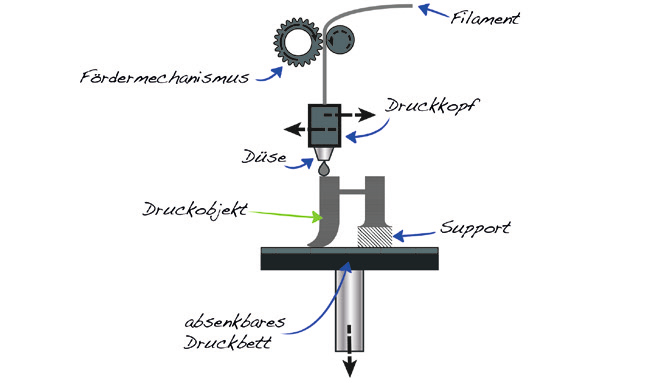
\includegraphics[width=0.9\textwidth]{chapter/main/img/fdm.png}
			\caption[Schematische Darstellung des FDM-/FFF-Verfahrens]{Schematische Darstellung
			einer möglichen Konfiguration des als FDM oder FFF bekannten 3D-Druck-Verfahrens. Ein
			Fördermechanismus (\emph{Extruder}) schiebt das Filament durch eine aufgeheizte Düse.
			Durch eine Bewegung der Düse und/oder des Druckbetts in mindestens 3 Achsen erfolgt
			eine Formung des gewünschten Objektes Ebene für Ebene. \cite[S. 114]{horsch20143d}}
			\label{fig:fdm}
		\end{figure}

		Das in dieser Arbeit beobachtete Verfahren ist jedoch das \emph{selektive Laserschmelzen}
		(SLM). Der Drucker besteht hierbei aus zwei Gefäßen mit beweglichen Böden (Abbildung
		\ref{fig:slm_sls}). Das Gefäß für den Materialvorrat (\emph{feed container}) ist mit dem
		Material in Pulverform gefüllt, während das andere wenig bis gar nicht gefüllt ist. Beim
		Drucken einer neuen Ebene hebt sich der Boden des Materialvorrats und eine Walze
		(\emph{Beschichtungseinheit}) überträgt das dosierte Material in den Druckraum, dessen
		Druckbett abgesenkt wird. Ein beweglicher Laser fährt nun die gewünschte Schnittebene ab
		und verschmilzt das Pulver zu einer festen Form \cite{horsch20143d}.
		%\todo[color=red]{Quelle dazu finden bzw. nennen. Florian Horsch?}

		\begin{figure}[!ht]
			\centering
			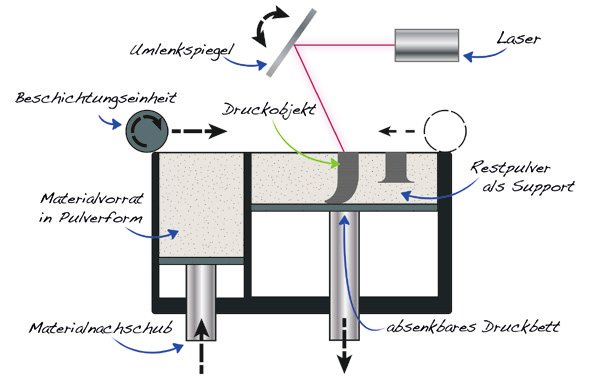
\includegraphics[width=0.9\textwidth]{chapter/main/img/sls_slm.png}
			\caption[Schematische Darstellung des SLM-Verfahrens]{Schematische Darstellung des
			SLM-Verfahrens. Der bewegliche Spiegel sorgt für eine präzise Positionierung des
			Laserpunktes. Während sich der Boden des Vorrats\-gefäßes im Prozess anhebt, senkt
			sich der Boden des Druckraums ab. \cite[S. 119]{horsch20143d}}
			\label{fig:slm_sls}
		\end{figure}

		Das Druckbett wird üblicherweise um \SI{30}{\micro\meter} bis \SI{100}{\micro\meter}
		abgesenkt \cite{song2012effects}, wobei diese Werte nicht als Minimal- oder Maximalwerte
		zu verstehen sind \cite{shi2016performance}. Zu den am häufigsten verwendete Materialien,
		die beim SLM-Verfahren verwendet werden, zählen Titanlegierungen, insbesondere das in der
		Luft- und Raumfahrt populäre Ti6Al4V
		\cite{song2012effects,shi2016performance,brandl2012morphology}. Aluminiumlegierungen
		werden ebenfalls verwendet \cite[je AlSi10Mg]{yan2020comparative,zou2017study}.

	\subsection{Beobachtbare Defekte im gefertigten Objekt}
		\subsubsection{Porenbildung}
		Aufgrund verschiedener physikalischer Phänomene treten während des Verfahrens Vorgänge auf,
		die sich in Defekten bemerkbar machen. Einer der bekanntesten Defekte ist die
		\emph{Porenbildung}. Mit einer Größe von weniger als \SI{100}{\micro\meter} zählen diese
		Gaseinschlüsse zu den kleinsten der hier aufgeführten Defekte \cite{zhang2017defect}. Es
		werden zwei verschiedene Gasquellen unterschieden. Während eine Quelle des dafür
		notwendigen Gases die Verdampfung mancher Legierungsbestandteile, wie beispielweise
		Magnesium, sein kann, kann ein Gaseinschluss nicht zuletzt auch durch Einschluss des beim
		Prozess verwendeten Umgebungsgases erfolgen \cite{galy2018main}. In letzterem Fall kann
		zum Beispiel eine zu geringe Packungsdichte des verwendeten Materialpulvers die Ursache
		sein. Das Gas dringt hierbei während des Schmelzprozesses in die Schmelze ein, erreicht
		aber aufgrund einer hohen Kühlrate die Oberfläche nicht vor dem Erstarren, sodass beim
		Erhärten des Materials ein Lufteinschluss die Folge ist. Aus diesem Grund haben Poren eine
		näherungsweise sphärische Form. Sie sind üblicherweise im im gefertigten Objekt
		gleichverteilt aufzufinden. Das komplette Eliminieren aller Poren gilt als sehr schwer
		\cite{zhang2017defect}. Galy et al. zufolge hat die Porengröße und -form einen
		entscheidenden Einfluss auf die Qualität des Endproduktes. Größere Makroporen
		verschlechtern die Qualität stärker als kleinere Mikroporen, wobei sich mehrere Mikroporen
		zu größeren Makroporen vereinigen können. Eine stärkere Entrundung der sphärischen Form
		der Poren kann eine Ursache von Rissen im Objekt sein \cite{galy2018main}. Poren
		unterschiedlicher Größe sind in Abbildung \ref{fig:defects_porosities} zu sehen.

		\begin{figure}[!ht]
			\centering
			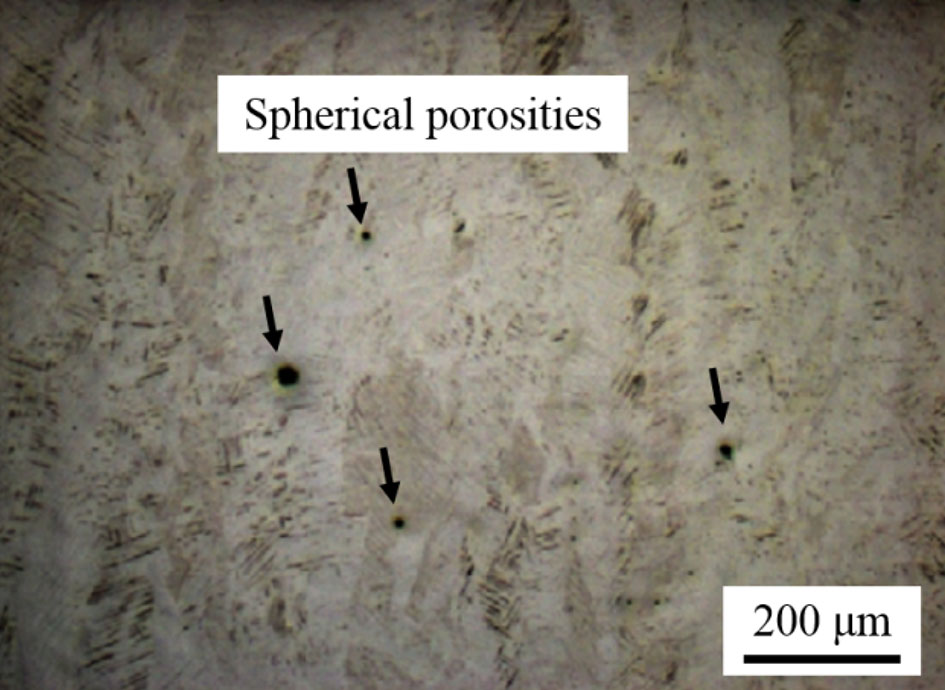
\includegraphics[width=0.6\textwidth]{chapter/main/img/defects/porosities.png}
			\caption{Poren sphärischer Form unterschiedlicher Größe entstehen durch Gaseinschlüsse
			\cite{zhang2017defect}}
			\label{fig:defects_porosities}
		\end{figure}

		\subsubsection{Mangelnde Verschmelzung}
		Eine mangelnde Verschmelzung (\emph{lack-of-fusion} oder kurz: \emph{LOF}) entsteht
		überwiegend durch unzureichende Energiezufuhr während des Schmelzprozesses. Durch die zu
		niedrige Energie vermindert sich die Breite des Schmelzbades. Bei unzureichender
		Überlappung der Bahnen kann dies zu fehlender Haftung zwischen diesen (sogenannten
		\emph{bonding defects} Abbildung \ref{fig:defects_lof} a)) führen. Außerdem resultiert
		die LOF in zahlreichen Pulvereinschlüssen (Abbildung \ref{fig:defects_lof} b)). Sollte die
		Energiezufuhr sogar unzureichend sein, um die gesamte Schichthöhe zu penetrieren, führt
		dies zu mangelhafter Bindung zwischen den Ebenen. Aus diesen Gründen sind Defekte die
		LOF betreffend hauptsächlich zwischen den Bahnen einer Ebene und zwischen den Ebenen
		selbst zu finden. Da diese Defekte eine raue Oberfläche erzeugen, wird der Materialfluss
		der nächsten Ebene ebenfalls gestört, sodass Zwischenebenendefekte auftreten können, die
		graduell durch mehrere Ebenen propagieren und somit Defekte zur Folge haben, die sich über
		mehrere Ebenen erstrecken. Legierungen mit oxidierbaren Bestandteilen wie AlSi10Mg können
		durch einen entstehenden Oxidfilm und der damit verbundenen verminderten Benetzbarkeit
		ebenfalls Probleme mit der Aneinanderbindung von Bahnen haben \cite{zhang2017defect}.

		\begin{figure}[!ht]
			\centering
			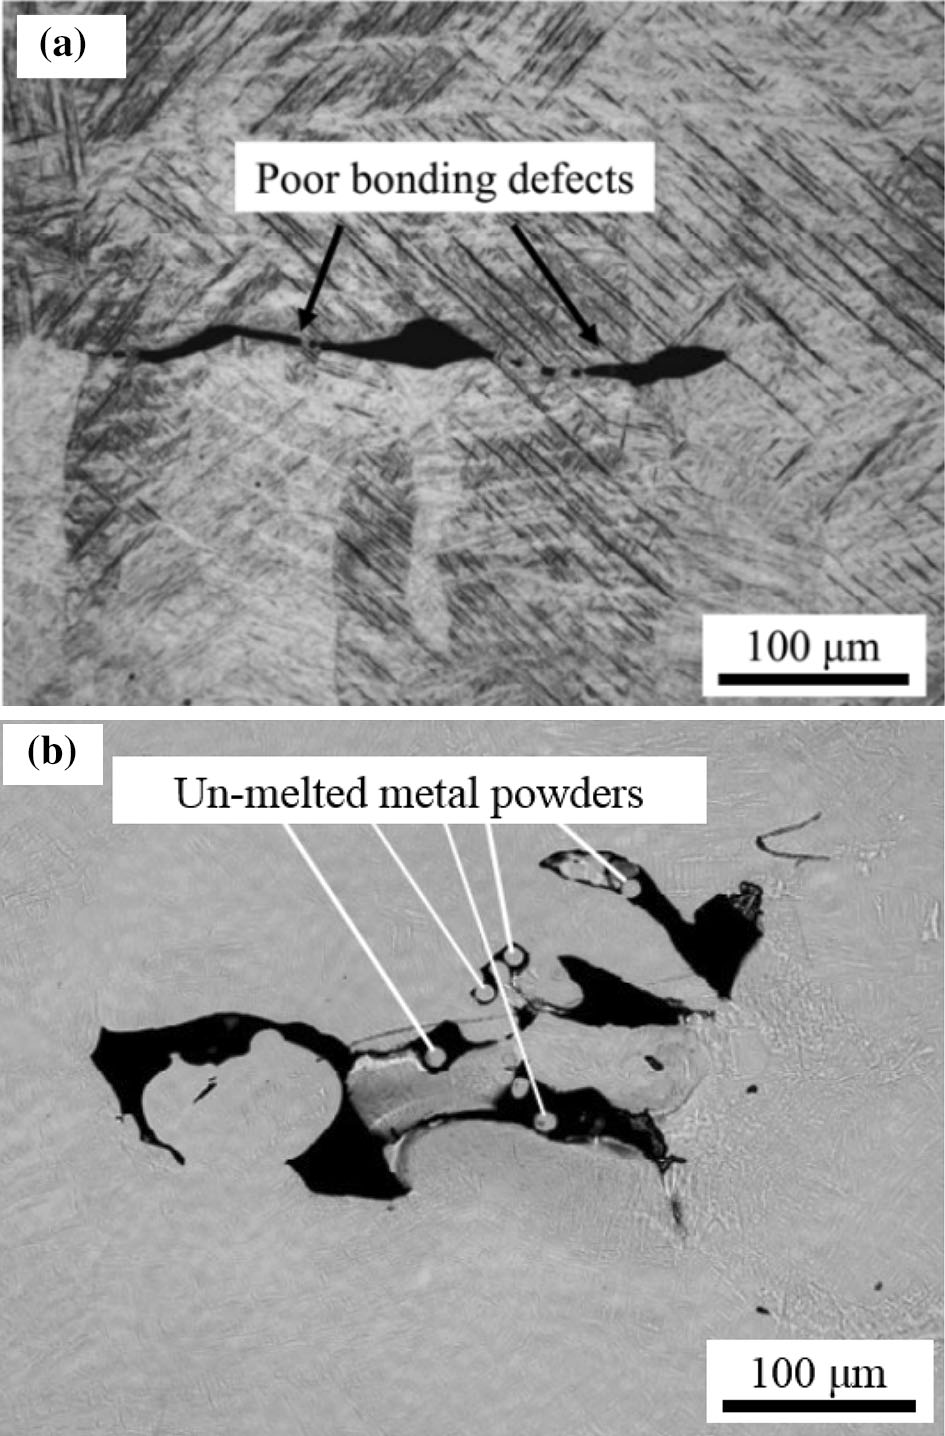
\includegraphics[width=0.6\textwidth]{chapter/main/img/defects/lack_of_fusion.png}
			\caption{a) Zwei Bahnen mit schlechter Verbindung durch mangelnde Überlappung
			b) Gut erkennbare Pulvereinschlüsse durch unzureichendes Aufschmelzen des Pulvers
			in Hohlräumen \cite{zhang2017defect}}
			\label{fig:defects_lof}
		\end{figure}

		\subsubsection{Risse}
		Während des Schmelzprozesses herrschen nach dem Schmelzen Kühlraten von bis zu
		\SI{e8}{\kelvin\per\second}. Der dadurch entstehende Temperaturgradient und die damit
		verbundene unterschiedlich starke Kompression führt zu hohen Spannungen im Material.
		Diese Spannungen können nun dafür sorgen, dass Risse (\emph{cracks}) entstehen und dass
		diese weiter durch das Material propagieren. Abbildung \ref{fig:defects_cracks} zeigt gut
		verschiedene Stellen eines Risses, der sich an einer Oberfläche gebildet hat und weiter in
		das gefertigte Objekt hineinpropagiert ist \cite{zhang2017defect}. Wie bereits in
		Abschnitt \emph{Porenbildung} erwähnt können auch nicht-sphärische Poren besonders
		begünstigend auf die Rissbildung wirken \cite{galy2018main}.

		\begin{figure}[!ht]
			\centering
			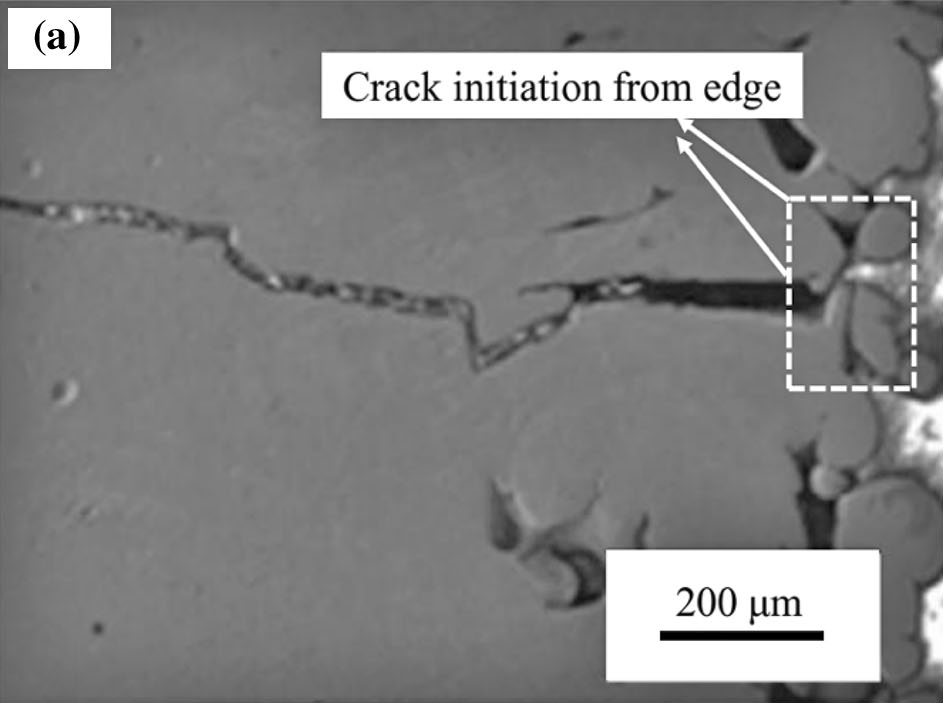
\includegraphics[width=0.6\textwidth]{chapter/main/img/defects/cracks_part.png}
			\caption{Aufnahme des Rands eines produzierten Objektes, von dem ein Riss ausgeht. Es
			ist gut erkennbar wie der Riss von Rand ausgehen in das Objekt hineinpropagiert ist.
			\cite{zhang2017defect}}
			\label{fig:defects_cracks}
		\end{figure}

		\subsubsection{Keyholes}
		Ssogenannte \emph{Keyholes} treten besonders bei hohen Temperaturen auf. In diesem Fall
		kann ein Teil des Materials vaporisieren und dann eine V-förmige Furche wie in Abbildung
		\ref{fig:defects_keyholes} zurücklassen.

		\begin{figure}[!ht]
			\centering
			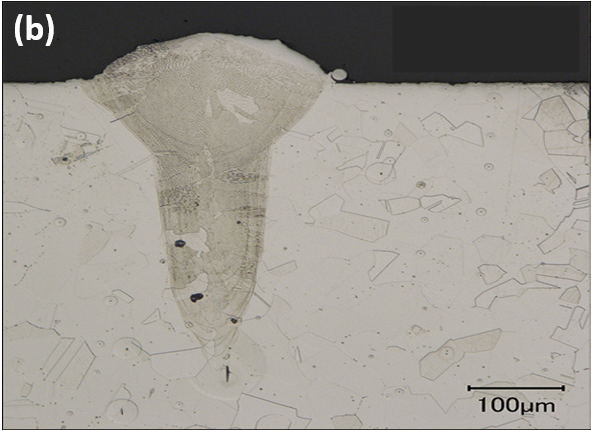
\includegraphics[width=0.6\textwidth]{chapter/main/img/defects/keyhole.png}
			\caption{Ein als Keyhole bekannter Defekt \cite{eskandarisabzi2019defect}}
			\label{fig:defects_keyholes}
		\end{figure}

	\subsection{Wichtige Parameter und Einfluss der Lasergeschwindigkeit}
		Beim SLM-Verfahren sind verschiedene Parameter einstellbar, die das Resultat in
		unterschiedlicher Weise und Stärke beeinflussen. Eine kategorische Übersicht über alle
		beim SLM-Prozess variierbaren Parameter ist in Abbildung \ref{fig:scheme_parameters} zu
		finden.

		\begin{figure}[!ht]
			\centering
			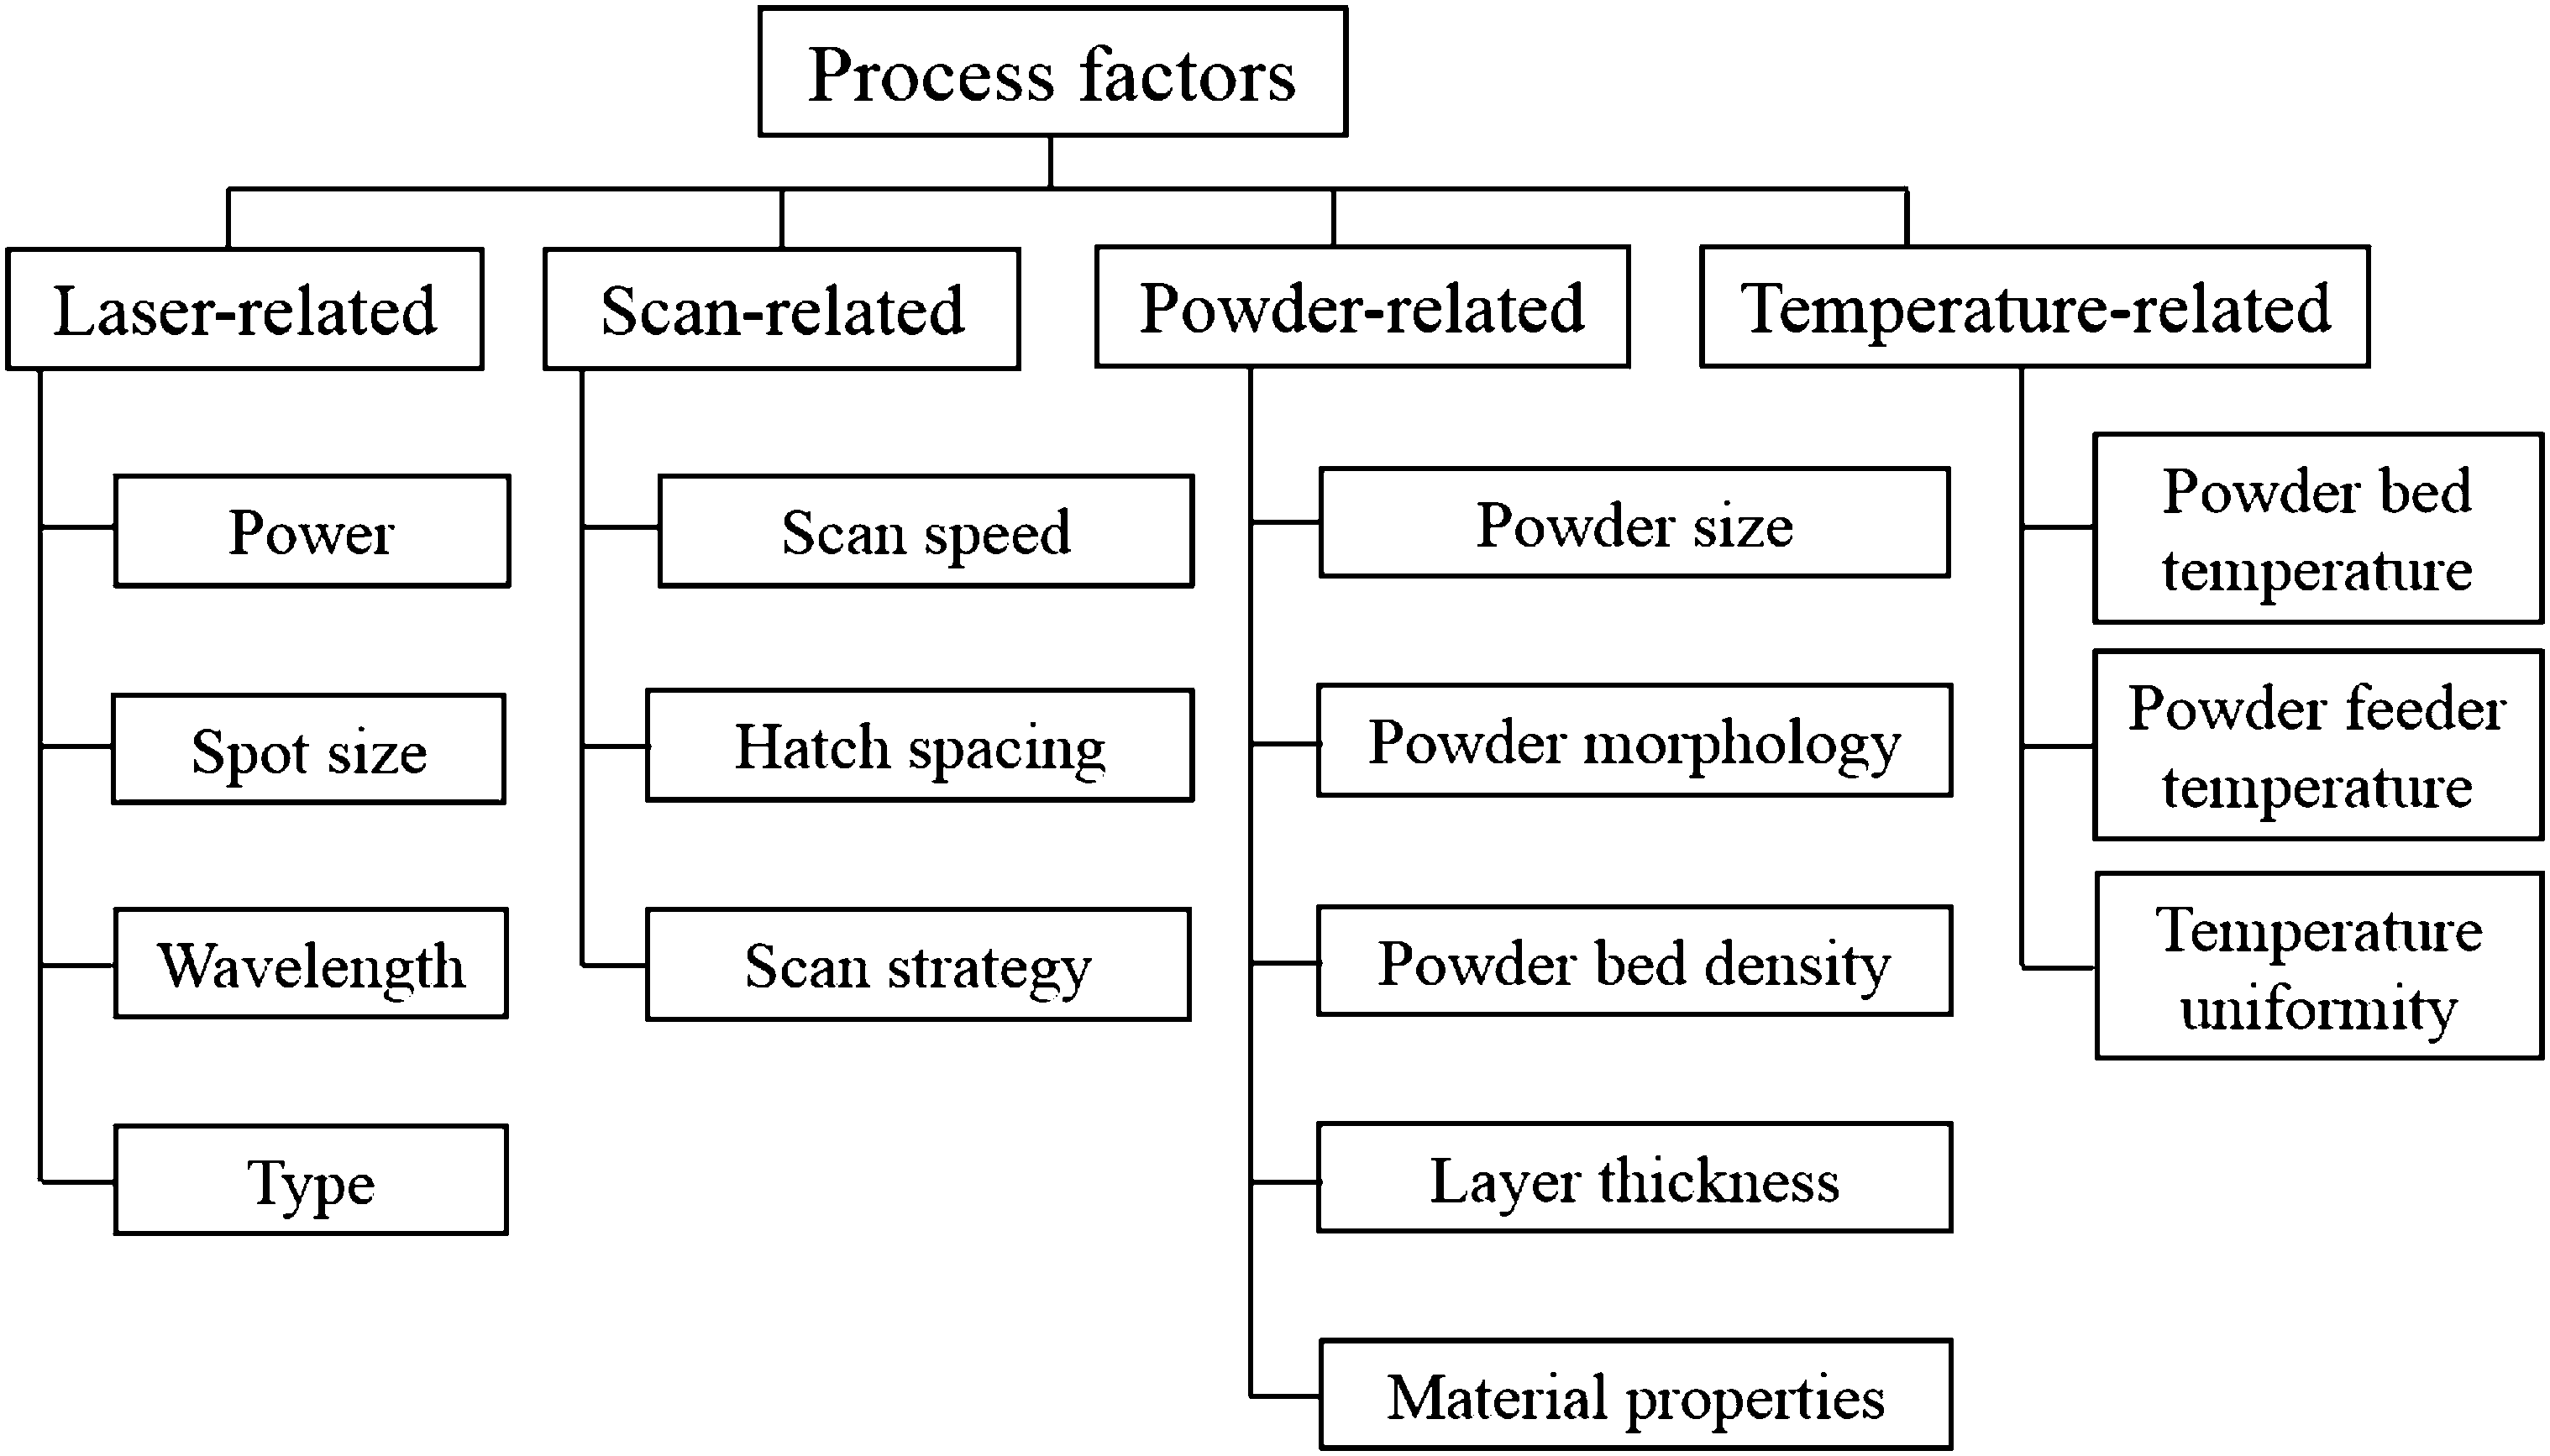
\includegraphics[width=0.9\textwidth]{chapter/main/img/scheme_parameters_2.png}
			\caption{Eine Übersicht aller beim SLM-Verfahren einstellbaren Parameter nach
			Kategorie geordnet \cite{zhang2017defect,aboulkhair2014reducing}}
			\label{fig:scheme_parameters}
		\end{figure}

		Die wichtigsten Parameter sind, wie in Abbildung \ref{fig:slm_parameters} zu sehen, die
		Lasergeschwindigkeit (\emph{scanning speed}), die Laserleistung, der horizontale
		Bahnabstand (\emph{hatch distance} oder \emph{hatch spacing}), die Wellenlänge des Lasers,
		der Durchmesser des fokussierten Laserpunktes (\emph{spot size}) und die durch die Dicke
		der Pulverschicht bestimmte Ebenenhöhe (\emph{layer thickness})
		\cite{sadali2020influence}. Da für diese Arbeit die Größenordnung im Bereich der einzelnen
		Pulverpartikel von Interesse ist, werden im weiteren Verlauf der Bahnabstand und die
		Ebenenhöhe nicht weiter betrachtet.

		\begin{figure}[!ht]
			\centering
			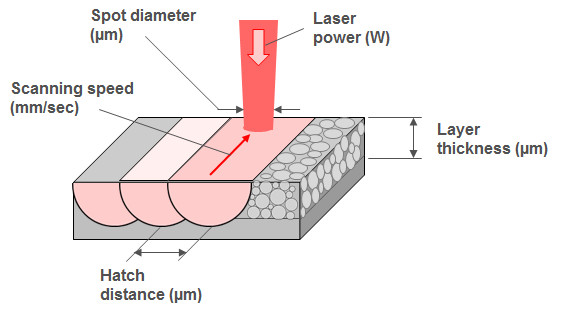
\includegraphics[width=0.9\textwidth]{chapter/main/img/slm_parameters.jpg}
			\caption{Darstellung und räumliche Einordnung der wichtigsten einstellbaren Parameter
			beim SLM-Druck und ihre üblichen Einheiten \cite{saunders2017x}}
			\label{fig:slm_parameters}
		\end{figure}

		Für ein optimales Ergebnis bedarf es natürlich einer optimalen Abstimmung der Parameter
		aufeinander. Beispielsweise ist für eine Erhöhung der Lasergeschwindigkeit oft eine
		größere Laserleistung nötig, um das Schnelzen des Materials weiterhin zu gewährleisten.

		Sadali et al. fanden heraus, dass mit steigender Lasergeschwindigkeit die Größe der Poren
		reduziert wird. Außerdem entstehen weniger Spritzer (\emph{splashing effect}). Anhäufungen,
		die bei der Auftrennung von instabilen Flüssigspuren durch mangelnde Benetzbarkeit
		entstehen können (\emph{balling effect}, Abbildung \ref{fig:defects_balling}), werden mit
		steigender Geschwindigkeit nicht nur weniger, sondern auch kleiner.

		\begin{figure}[!ht]
			\centering
			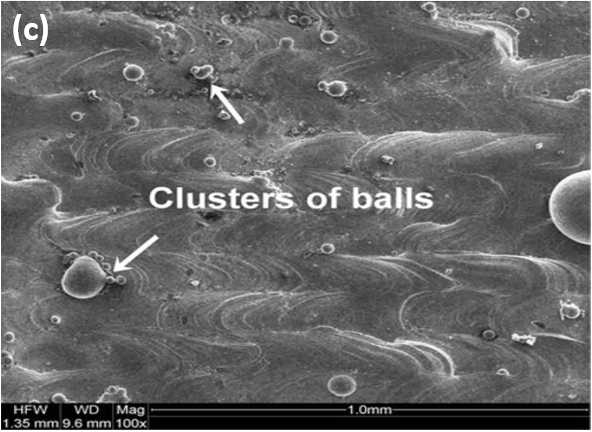
\includegraphics[width=0.7\textwidth]{chapter/main/img/defects/balling.png}
			\caption{Der sogenannte \emph{balling effect} entsteht, wenn die Benetzbarkeit der
			darunter liegenden Schicht nicht ausreicht, sodass sich aus dem geschmolzenen
			Material kugelförmige Ansammlungen bilden \cite{eskandarisabzi2019defect}}
			\label{fig:defects_balling}
		\end{figure}

		Nichtsdestotrotz bedeutet dies nicht unbedingt, dass ein schnellerer Laser grundsätzlich
		ein bisseres Gesamtergebnis erzielt. Mit höherer Geschwindigkeit treten beispielsweise
		auch mehr Mikrorisse auf. Während diese durch \emph{Heißisobarisches Pressen} (\emph{HIP})
		zwar minimiert werden können, treten ab einer gewissen Geschwindigkeit jedoch vermehrt
		Keyholes auf, deren nachträgliche Reduktion durch HIP nicht möglich ist
		\cite{sadali2020influence}.


\section{Molekulardynamische Modellierung von SLM}
	\subsection{Grundlegende Funktionsweise der Molekulardynamik (MD)}
		Um die Trajektorien aller Teilchen in einem System großer Teilchenzahl $N$ zu bestimmen,
		bedarf es der Lösung der zugehörigen Bewegungsgleichungen, wie sie in Gleichung
		\eqref{eq:newtone_dgl} zu sehen sind.

		\begin{align}
			m_i \ddot{\uvec{x}}_i &= \uvec{F}_i
			& \text{mit} &&
			\uvec{F}_{i} &= \sum_{\substack{j=0\\j \neq i}}^{N-1} \uvec{F}_{ij}
			= -\sum_{\substack{j=0\\j \neq i}}^{N-1} \nabla_i U_j = -\nabla_i U
			\label{eq:newtone_dgl}
		\end{align}

		Hierbei ist $m_i$ die Masse des Teilchens $i$, $\uvec{x}_i$ der Ortsvektor von diesem und
		$\uvec{F}_{i}$ die vektorielle Gesamtkraft auf dieses. Weiterhin ist $\uvec{F}_{ij}$ die
		Einzelkraft zwischen zwei Teilchen $i$ und $j$ sowie $U_i$ das vom Teilchen $i$ ausgehende
		Potential und $\nabla_i$ der Gradient in der Koordinate $\uvec{x}_i$. Da diese
		Bewegungsgleichungen für große Teilchenzahlen $N$ im Allgemeinen nicht analytisch lösbar
		sind, %\todo[color=green]{Bezug auf NLD-Vorlesung bzgl. Unlösbarkeit?}
		bedarf es einer Simulation zur numerischen Integration dieser.

		Bei der Molekulardynamik (\emph{MD}) werden also Systemeigenschaften explizit anhand der
		zugrundeliegenden Wechselwirkung zwischen den Teilchen bestimmt, indem in einem
		iterativen Verfahren alle Bewegungsgleichungen explizit gelöst werden. Das bedeutet
		konkret: In einem Schritt werden die Kräfte $F_{ij}$, die von allen anderen Teilchen
		$j \neq i$ auf ein Teilchen $i$ wirken errechnet. Im nächsten Schritt resultieren daraus
		die nächsten Werte der Phasenraumkoordinaten. Um eine gewisse Zeitspanne $t$ zu
		beschreiben wird dieser Vorgang nun mehrmals iterativ wiederholt
		\cite{allen2004introduction}. Abbildung \ref{fig:scheme_md} erläutert die Vorgehensweise
		am Beispiel eines beliebigen Teilchens in direkter Umgebung weniger anderer Teilchen.

		\begin{figure}[!ht]
			\centering
			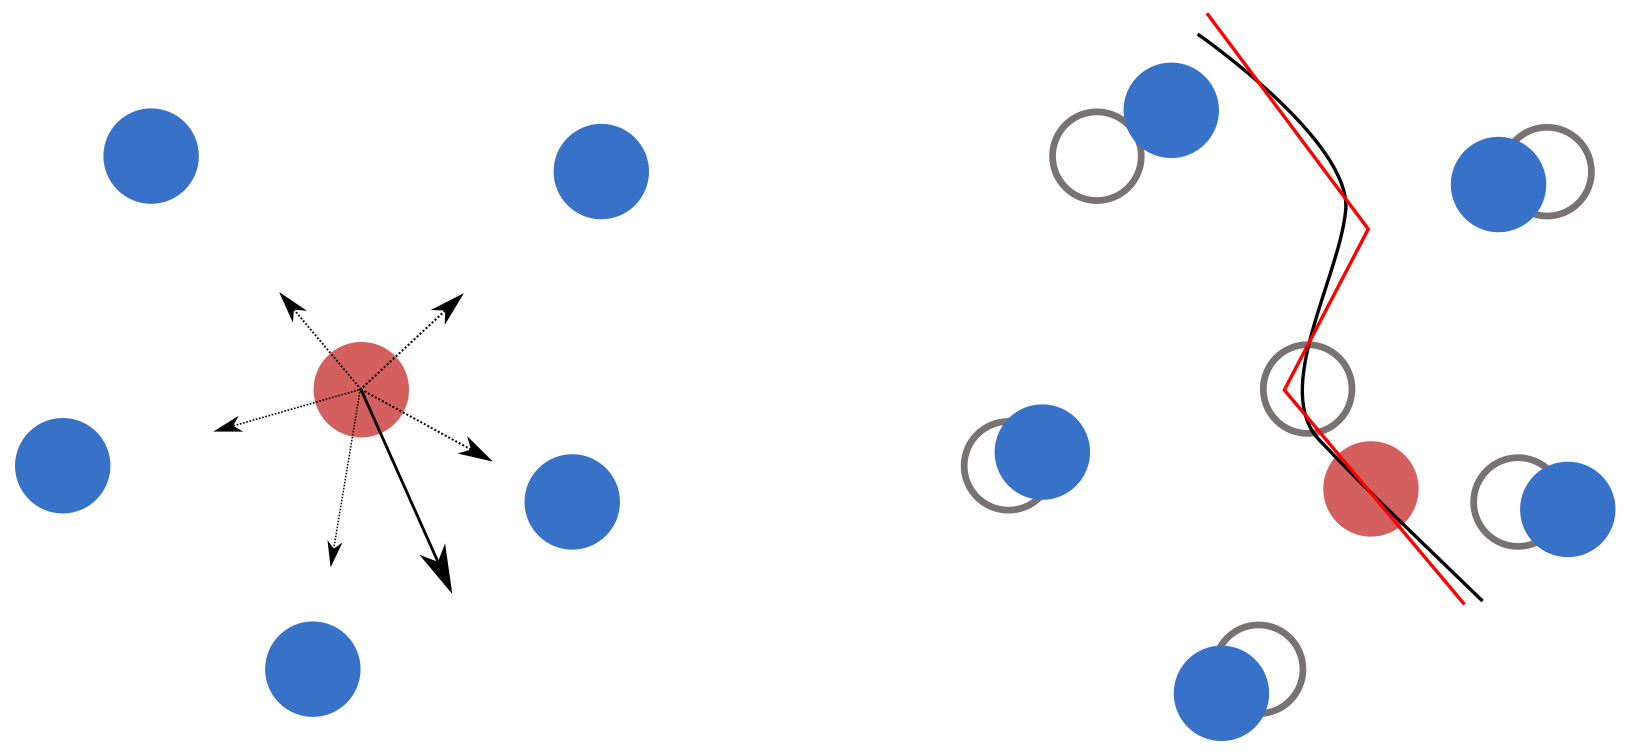
\includegraphics[width=0.8\textwidth]{chapter/main/img/scheme_md.png}
			\caption{Schematische Darstellung der Trajektorienerstellung bei der klassischen
			Molekulardynamik mithilfe eines beliebigen iterativen Integrators. Im ersten Schritt
			(links) wird die auf das rote Teilchen wirkende Gesamtkraft bestimmt. Gleiches
			passiert auch für die anderen Teilchen. Im nächsten Schritt (rechts) werden nun alle
			Teilchen entsprechend der auf sie wirkenden Kräfte verschoben und bilden somit in
			guter Näherung die Trajektorie der jeweiligen Teilchen.
			\cite[S. 52]{sonntag2011computer}}
			\label{fig:scheme_md}
		\end{figure}

		Das am weitesten verbreitete Potential für klassische Molekulardynamik mit ungeladenen
		Teilchen ist das Lennard-Jones-Potential nach Gleichung \eqref{eq:potential_lj}.

		\begin{align}
			U^\text{LJ}(r) &= 4\epsilon \left[
				\left(\frac{\sigma}{r}\right)^{12}
				-
				\left(\frac{\sigma}{r}\right)^{6}
			\right] \label{eq:potential_lj}
		\end{align}

		Wie in Abbildung \ref{fig:potential_lj} zu sehen besteht es aus einer stärkeren, aber
		kurzreichweitigen, attraktiven Komponente und einer schwächeren, aber langreichweitigeren,
		attraktiveren Komponente.

		\begin{figure}[!ht]
			\centering
			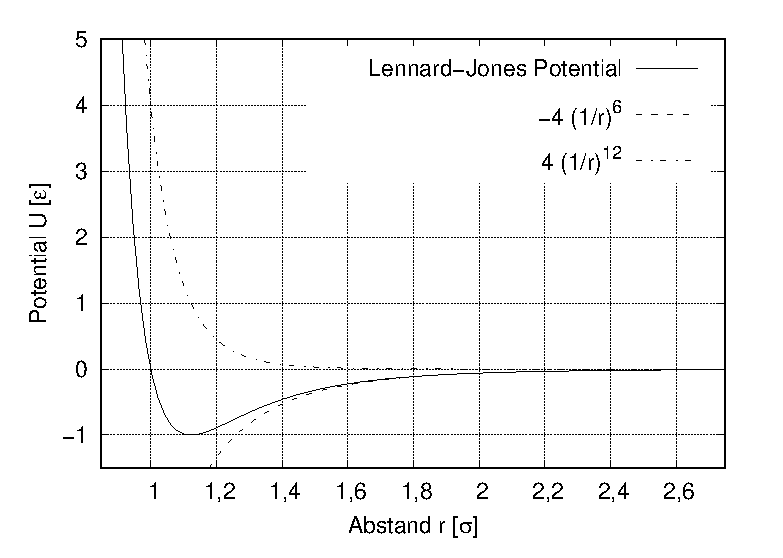
\includegraphics[width=0.8\textwidth]{chapter/main/plt/lennard_jones.eps}
			\caption{Auftragung der Funktion in Gleichung \eqref{eq:potential_lj} in Einheiten
			der Parameter $\epsilon$ und $\sigma$}
			\label{fig:potential_lj}
		\end{figure}

		Da die aus dem Potential folgende Kraft lediglich entlang des Richtungsvektors
		$\uvec{r}_{ij} = \uvec{x}_j - \uvec{x}_i$ wirkt, ist eine rein radiale Betrachtung in
		Kugelkoordinaten nach Gleichung \eqref{eq:force_lj} ausreichend. Da für jedes der $N$
		Teilchen $N-1$ Einzelkräfte berechnet werden müssen, skaliert die Anzahl der Berechnungen
		mit $N(N-1)$ ($\rightarrow N^2$ für große $N$). Durch Newtons drittes Gesetz
		$\uvec{F}_{ij} = -\uvec{F}_{ji}$ lässt sich die Anzahl der expliziten Kraftberechnungen
		halbieren, wobei das Skalierungsverhalten weiterhin quadratisch bleibt.

		\begin{align}
			\uvec{F}_{ij} &= -\nabla_i U^\text{LJ}\left(
				\left\|\uvec{x}_i - \uvec{x}_j\right\|
			\right) \nonumber
			&\Rightarrow&&
			F_{ij}(r) &= 24\epsilon \frac{\uvec{r}_{ij}}{r^2} \left[
				2\left(\frac{\sigma}{r}\right)^{12}
				-
				\left(\frac{\sigma}{r}\right)^{6}
			\right] \label{eq:force_lj}
		\end{align}

	\subsection{Reduzierte Einheiten}

	\subsection{Numerische Integration von newtonschen Bewegungsgleichungen}
		Die wohl simpelste Methode der numerischen Integration ist das \emph{Euler-Verfahren}.
		Hierbei wird das Taylorpolynom ersten Grades der Trajektorie verwendet und alle höheren
		Terme verworfen. Mithilfe der Diskretisierung des Zeitschritts \dt lässt sich von einem
		Integrationsschritt $n$ näherungsweise auf den nächsten $n+1$ schließen:

		\begin{align}
			\uvec{x}_{n+1} &= \uvec{x}_n + \dot{\uvec{x}}_n \dt + \BigO\left(\dt^2\right)
		\end{align}

		Hierbei bezeichnet $\dot{\uvec{x}}$ die erste Ableitung von $x$ nach der Zeit,
		$\ddot{\uvec{x}}$ die zweite Ableitung, und so weiter. Das Problem, welches dem
		Euler-Verfahren innewohnt, ist die Tatsache, dass es nicht symplektisch ist und somit
		nicht die für ein mikrokanonisches Ensemble notwendige Forderung nach Energieerhaltung
		erfüllen kann \cite[S. 6f]{klein2013klassische}.

		Ein symplektischer Algorithmus ist der \emph{Verlet-Algorithmus}. Er entsteht durch zwei
		Taylorentwicklungen 4. Ordnung der Trajektorie wie in den Gleichungen
		\eqref{eq:verlet_taylor_fw} und \eqref{eq:verlet_taylor_bw}, wobei eine der Entwicklungen
		mit positivem Zeitschritt \dt und eine mit negativem Zeitschritt -\dt durchgeführt wird
		\cite[S. 69f]{frenkel2001understanding}:

		\begin{align}
			\uvec{x}_{n+1} &= \uvec{x}_n + \dot{\uvec{x}}\dt + \frac{1}{2}\ddot{\uvec{x}}\dt^2
				+ \frac{1}{3!}\dddot{\uvec{x}}_n\dt^3 + \BigO\left(\dt^4\right)
				\label{eq:verlet_taylor_fw} \\
			\uvec{x}_{n-1} &= \uvec{x}_n - \dot{\uvec{x}}\dt + \frac{1}{2}\ddot{\uvec{x}}\dt^2
				- \frac{1}{3!}\dddot{\uvec{x}}_n\dt^3 + \BigO\left(\dt^4\right)
				\label{eq:verlet_taylor_bw}
		\end{align}

		Durch Addition ergibt sich damit ein nicht-selbststartender symplektischer Algorithmus wie
		in Gleichung \eqref{eq:verlet} beschrieben.

		\begin{align}
			\uvec{x}_{n+1} &= 2 \uvec{x}_n - \uvec{x}_{n-1} + \ddot{\uvec{x}}_n\dt^2
				+ \BigO\left(\dt^4\right) \label{eq:verlet}
		\end{align}

		Wie auch in der für diese Arbeit genutzten Simulationssoftware \emph{IMD}
		\cite{stadler1997imd} wird jedoch für MD-Simulationen häufig der zum Verlet-Verfahren
		äquivalente und selbststartende \emph{Velocity-Verlet-Algorithmus} aus Gleichung
		\eqref{eq:velocity_verlet} verwendet. Durch die Äquivalenz der beiden Algorithmen bleibt
		die symplektische Natur erhalten, jedoch ist der Algorithmus nun geschwindigkeitsabhängig.
		In der klassischen MD ist dies jedoch kein Problem, da die Geschwindigkeiten ohnehin von
		Interesse für manche Größen (wie beispielsweise die Temperatur des Systems) sind.

		\begin{align}
			\uvec{x}_{n+1} &= \uvec{x}_n + \dot{\uvec{x}}\dt
				+ \frac{1}{2}\ddot{\uvec{x}}\dt^2 + \BigO\left(\dt^4\right) \nonumber\\
			\dot{\uvec{x}}_{n+1} &= \dot{\uvec{x}}_n + \frac{\ddot{\uvec{x}}_n +
				\ddot{\uvec{x}}_{n+1}}{2}\dt + \BigO\left(\dt^2\right)
				\label{eq:velocity_verlet}
		\end{align}

	\subsection{Implementierung des Lasers}
		Bestrahlt man ein Material mit einem Laser, so regen die Photonen die Schwingungszustände
		der Atome an und sorgt somit dafür, dass sich das Material lokal aufheizt
		\cite{zhigilei1997velocity}. Nach Gleichung \eqref{eq:avg_kin_energy} ist hierbei die
		mittlere kinetische Energie $\left\langle E_\text{kin} \right\rangle$ proportional zur
		Temperatur $T$, wobei $f$ die Anzahl der Freiheitsgrade und $k_\text{B}$ die
		Boltzmannkonstante ist.

		\begin{align}
			\left\langle E_\text{kin} \right\rangle &= \frac{f}{2} k_\text{B} T
				\label{eq:avg_kin_energy}
		\end{align}

		Die wohl direkteste Implementierung des Aufheizens durch einen Laser ist also das
		Skalieren der Teilchengeschwindigkeiten gemäß eines durch Gleichung
		\eqref{eq:avg_kin_energy} geforderten Faktors für die Geschwindigkeiten. Sei nun die
		gewollte Energieänderung $\dx[E]$. Mit $E_\text{kin} \propto \dot{\uvec{x}}^2$ folgt
		also für den Faktor mit $\dot{\uvec{x}}(t + \dt) = a\dot{\uvec{x}}(t)$

		\begin{align}
			a^2 &= \frac{E_\text{kin}(t + \dt)}{E_\text{kin}(t)}
			&\Rightarrow&&
			a &= \sqrt{\frac{E_\text{kin}(t) + \dx[E]}{E_\text{kin}(t)}}
				= \sqrt{1 + \frac{\dx[E]}{E_\text{kin}(t)}}
		\end{align}

		Da $E_\text{kin}(t)$ durch Summation aller Geschwindigkeitsquadrate einfach bestimmt
		werden kann, bleibt als unbekannte die gewünschte Einbringung $\dx[E]$. Um diese zu
		bestimmen wird ein gaußförmiges Intensitätsprofil nach Gleichung \eqref{eq:gauss_profile}
		angenommen.

		\begin{align}
			I(x,y) = I(r) &= I_0 \exp\left(-a r^2\right) \label{eq:gauss_profile}
		\end{align}

		Es gilt $a = \frac{1}{2\sigma^2}$, wobei $\sigma$ die Varianz der Gauß-Funktion ist.
		Wird die Gauß-Funktion normiert, so hängt der Vorfaktor, und damit auch die Höhe der
		Funktion, von der Varianz, und damit von der Breite der Funktion, ab
		(Abbildung \ref{fig:gauss}).

		\begin{figure}
			\centering
			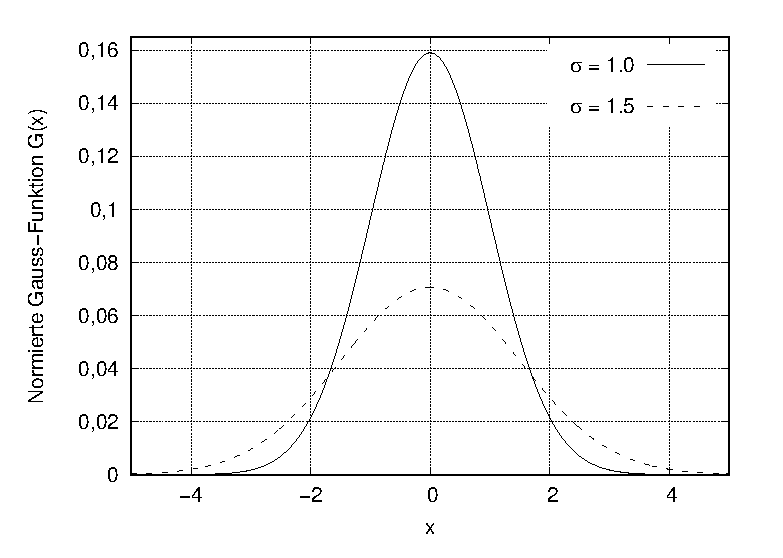
\includegraphics[width=0.8\textwidth]{chapter/main/plt/gauss.eps}
			\caption{Eine auf 1 normierte Gauß-Funktion wird mit abnehmender Breite höher und
			umgekehrt}
			\label{fig:gauss}
		\end{figure}

		Es ist offensichtlich, dass das Profil nur von der radialen Komponente $r$ der
		zylindrischen Koordinaten entlang der Strahlrichtung abhängig ist. Für einen Laser in
		$z$-Richtung ist $r^2 = x^2 + y^2$. Eine Integration entlang der Ebene senkrecht zur
		Strahlrichtung muss die Gesamtleistung $P_\text{Ges}$ des Lasers ergeben.

		\begin{align}
			P_\text{Ges} &= \int_{\mathbb{R}^2} I(r) \dx\dx[y]
				= I_0 \int_0^{2\pi} \dx[\theta] \int_0^\infty \exp\left(-a r^2\right) \dx[r]
		\end{align}

		Drückt man die Varianz nun als Halbwertsbreite $\fwhm = 2\sqrt{2 \ln2}\sigma$ aus, so
		ergibt sich für die maximale Intensität $I_0$

		\begin{align}
			I_0 &= \frac{P_\text{Ges}}{\pi} \frac{4\ln2}{\fwhm^2}
		\end{align}

		Da in der Herleitung bisher noch keine Intensitätsabschwächung nach dem
		\emph{Lambert-Beer-Gesetz} mit der Absorption $\mu$ erfolgt ist, wird die Intensität mit
		dem entsprechenden Faktor multipliziert. Ebenso wird direkt der Reflexionskoeffizient
		$R$ mit eingebunden.

		\begin{align}
			I(x,y,z) &= \exp\left(-\mu z\right) \cdot (1-R) \cdot I(x,y)
			\label{eq:intensity}
		\end{align}

		Um daraus nun die diskrete Energieänderung $\dx[E]$ zu erhalten, bedarf es einer
		Betrachtung der Größen pro diskreter Volumeneinheit $\dx[V]$ und pro Zeitschritt $\dt$:

		\begin{align}
			\dx[I] &= \frac{\dx[E]}{\dx[A]\cdot\dt}
			&\Leftrightarrow&&
			\dx[E] &= \dx[I] \cdot \dx[A] \cdot \dt
		\end{align}

		Erweitern mit $\dx[z]/\dx[z]$ führt nun auf die Form in Gleichung
		\eqref{eq:energy_diff_1}.

		\begin{align}
			\dx[E] &= \frac{\dx[I]}{\dx[z]} \cdot \dx[z] \cdot \dx[A] \cdot \dt
				= \frac{\dx[I]}{\dx[z]} \cdot \dx[V] \cdot \dt
			\label{eq:energy_diff_1}
		\end{align}

		Zwar ist $\dx[I]/\dx[z]$ ein Differenzenquotient, im diskreten Kontext aber kommt diesem
		die gleiche Bedeutung wie die Ableitung $\partial_z I$ zu. Diese ist durch Gleichung
		\eqref{eq:intensity} bekannt, sodass der Gesamtausdruck für die Energieänderung nun

		\begin{align}
			\dx[E] &= (1-R) \cdot \mu \cdot \exp\left(-\mu z\right)
				\cdot \frac{P_\text{Ges}}{\pi \sigma_\text{sc}^2}
				\cdot \exp\left(-\frac{x^2 + y^2}{\sigma_\text{sc}^2}\right)
				\cdot \dx[V] \cdot \dt
		\end{align}

		lautet. Zu beachten ist, dass $\sigma_\text{sc}^2 = 2\sigma^2 = \fwhm^2/(4\ln2)$ nicht die
		Varianz ist, sondern nur der übersichtlicheren Darstellung dient.

	\subsection{Näherungen und Vereinfachungen}
		%\todo[color=red]{Implementierung des Lasers: Lambert-Beer-Gesetz wie es implementiert ist eigtl nur für ebene Oberflächen gültig.}
		\subsubsection{Lambert-Beer'sches Gesetz}
		Eine Näherung, die aus Gründen der einfacheren Implementierung und der besseren
		Rechenleistung sinnvoll ist, ist eine vereinfachte Anwendung des Lambert-Beer'schen
		Gesetzes. Während bei diesem Gesetz eigentlich die Länge betrachtet wird, während der sich
		die elektromagnetischen Wellen tatsächlich im Medium befinden, wird hier für den Eintritt
		der Absorption ein fixer $z$-Wert angenommen. Dies hat den Grund, dass eine Absorption
		nach exakten Maßstäben nur durch eine Diskretisierung des Lasers in kleinere Unterstrahlen
		und eine darauf aufbauende Strahlverfolgung (\emph{Raytracing}) möglich wäre. Dies ist
		jedoch sehr rechenintensiv und müsste zudem nach jedem Simulationsschritt wiederholt
		werden. Weil diese Näherung für Geometrien mit in $z$-Richtung homogener Atomverteilung
		und gerader Oberkante (zum Beispiel quader- oder zylinderförmige Objekte) exakt ist, kann
		sie als annehmbare Näherung für kugelförmige Anordnungen, wie sie hier verwendet werden,
		gesehen werden. Zwar führt dies zu einer Änderungen in den Einzeltrajektorien, jedoch ist
		eine Änderung der makroskopischen Eigenschaften nicht zu erwarten, da die Dynamik des
		System näherungsweise gleich bleibt.

		\todo[color=red]{Kurzes Kapitel darüber warum Aluminium bzw über Alu an sich. zB AluSi10Mg
		enthält nach DIN EN 1706 ca. 90 \% Alu}
		%\todo[color=red]{Kleinere Skala und größere Gravitation mithilfe von \cite{glosli2007extending} motivieren.}
		\subsubsection{Änderungen der Größenordnungen}
		Für die Simulationen werden im Folgenden die Größenordnungen kleiner skaliert. Während die
		Partikelgröße der Pulverpartikel beim SLM-Verfahren üblicherweise im Bereich von wenigen
		Mikrometern \cite{hajnys2020research} was mit den bisherigen Errungenschaften der MD nur
		schwer zu schaffen ist \cite{eckhardt2013scientists}. Aus diesem Grund wird eine
		Pulverpartikelgröße in der Größenordnung der hunderten Nanometer angenommen. Dies wird
		durch eine Veröffentlichung von Glosli et al. motiviert. Diese Forschungsgruppe hat
		die Kelvin-Helmholtz-Instabilität bei verhältnismäßig kleiner Teilchenzahl als Ergebnis
		ihrer Simulation nachweisen können. Weil eben diese Instabilität stark von ihren
		Anfangswerten auftritt kann dies als Motivation verstanden werden den hier zu simuliernden
		Sachverhalt ebenfalls auf kleinere Maßstäbe zu schrumpfen, da hier im wesentlichen ebenfalls
		das Verhalten von Fluiden von Interesse ist \cite{glosli2007extending}. Wie in dieser
		Veröffentlichung muss hier als Ausgleich dazu ebenfalls die Gravitation erhöht werden.

	%\subsection{Besonderheiten bei der Simulationssoftware IMD}
